\documentclass[practical,english]{info1thesis}
% possible types: seminar, practical (bachelor, master, zula)
% Für Bachelor-, Master-, und Zulassungsarbeiten die Vorlage my-bachelor-master-zula.tex verwenden!
% possible languages: english, german

\usepackage[utf8]{inputenc}
\usepackage[T1]{fontenc}
\usepackage{lmodern}
\usepackage{placeins}

\graphicspath{{figures/}}


%%%%%%%%%%%%%%%%%%%%%%%%%%%%%%%%%%%%%%%%%%%%%%%%%%%%%%%%%%%%%%%%%%%%%%%%%%
%%%%%%%%%%%%% Bitte nur ab hier Änderungen vornehmen %%%%%%%%%%%%%%%%%%%%%

\title{Creating a Graph Harvester} % Geben Sie hier den Titel Ihrer Arbeit an.

\author{Jonas Spies} % Geben Sie Ihren Namen an.
\semester{Summer semester 2026}
\submissiondate{}
\supervisors{% Geben Sie die Namen aller Betreuer ab, getrennt durch das Makro '\and'
Prof.\ Dr.\ Alexander Wolff \and
Tim Hegemann, M.\,Sc.
} 


\begin{document}
\tableofcontents
\newpage
\begin{abstract}
In an attempt to answer the question of what makes a graph interesting, House of Graphs have built a database of many interesting graphs.
However manual insertion of new graphs being tedious creates the need for an application that automates this process.
While such a system already existed, it suffered from the necessity of hosting a server due to the project being written in Python and a relatively low detection rate:
Mooney, Hegemann, Wolff, Wybrow and Purchase counted roughly 40\% of the extracted graphs as satisfactory.
Thus, I have rebuilt a similar application in Typescript to allow client-side execution while deviating from the original workflow in some aspects in the hope of improving the detection rate.
Using graph drawings from papers featured in the International Symposium on Graph Drawing and Network Visualization from 1998 to 2024, I estimated the new implementation's performance against that of the old one, and came to the conclusion that the two systems' detection rates are similar.
The main reason why further improvement may be difficult is the trade-off that arises with the adjustment of some parameters: if they are changed to properly detect one instance, another instance may not be able to be detected correctly.    
\end{abstract}
\newpage

\section{Introduction}
Graph theory is a major field in mathematics and computer science due to a graph's ability to represent objects and their relations to each other in a compact and intuitive manner.
This representation allows all kinds of problems to be solved in a unified approach, such as the problem of finding the shortest path from one location to another, as often applied in navigational devices.


Many of these graphs may have certain properties that make them inherently more interesting than others. 
For example, they may serve as a particularly illustrative example to show an algorithm's best or worst case performance, as a counterexample to a plausible conjecture, or as an extreme instance where some property, for example planarity, still holds.
While it remains difficult to define what makes a graph ``interesting'', we use the appearance of a graph in a scientific paper as a major indicator for potential interest, leading our focus on to graphs featured in them.


In an attempt to give the word ``interesting'' a more concrete meaning, House of Graphs (HoG)\footnote{https://houseofgraphs.org/} have made it their mission to create a database that contains many such graphs.
However, scanning through hundreds of papers manually is not only prone to errors especially for large graphs, but also very time consuming, which is why we aimed to write a program that can automate this process.


Thus, a graph harvester app has been developed in Python to automatically scan scientific papers and heuristically extract any graph contained in them in a vector format, returning a visualization, a Graph6 String, and a link to the respective database entry or to the upload form for that graph.
A user can then use this tool to upload new graphs with the click of a button.


I have rebuilt the project in Typescript to allow client-side execution of the code, thus eliminating the need of hosting a server.
This opens up the possibility of integrating the harvester into the website of HoG, while achieving similar performance compared to that of the previous system.
For visualization, I reused the existing frontend built with React.
While following the general work pipeline of the previous implementation, I allowed myself to deviate from it by also adding and omitting a selected number of processing steps.
For example, I widened the definition of a vertex from ``a rectangle or a circle'' to ``any object of limited complexity that forms a closed loop''. 
Changes like this, however, also come with new problems, for instance arrow heads being treated as vertices and such.


Using papers featured in the International Symposium on Graph Drawing and Network Visualization\footnote{https://graphdrawing.unipg.it/} from 1998 to 2024 to measure progress during development, I have also made some observations about the general structure of these papers and their respective graph drawings, as well as on what makes a graph drawing ``difficult'' to scan heuristically.
Furthermore, I will highlight several trade-offs one has to consider when adjusting the system's parameters.


These observations could serve as a starting point for anybody aiming to improve the project, or as a guideline on how to make machine-readable graph drawings for researchers who wish to find their graphs included in the HoG database.

\section{System Limitations}
In order to scan graphs, we limit ourselves to vector graphics because those consist of multiple drawn objects that can be examined heuristically to discern between vertices and edges.
While the ability to scan bitmaps as well could be promising, this would require additional effort such as working with convolutional neural networks to extract patterns.
With only roughly 17\% of the figures in the dataset -- manually evaluated by~\cite{mooney_et_al:LIPIcs.GD.2025.30} -- being drawn as a bitmap, we deemed the extra effort not worth it, although future work may easily improve the performance by supporting bitmaps as well.


Besides that, we limit ourselves to undirected, simple graphs, so that any two vertices $u,v$ with an edge from $u$ to $v$ also contains an edge from $v$ to $u$. 
This information is stored in a single edge $(u,v)$ (or alternatively $(v,u)$), and each pair of vertices can only have up to one edge in the graph.
While there may also be many interesting directed graphs or multigraphs, House of Graphs does not support them, thus we do not discern between them.


Lastly, there are many graph drawings that only include four or less vertices. 
While one could argue that such graphs are interesting as well, the likelihood of that instance already being on the database is high, which is why we limit ourselves to graphs that have at least five vertices, four edges, and no isolated vertices (isolated vertices will just not be considered part of the graph during detection).

\section{Previous Work}
In this segment I will give a short overview over how the previous harvester works and its limitations.
\subsection{Workflow}
The old implementation handles one document at a time, going through that document page by page.

\paragraph{Identifying Figures}
As a first step on each page, the old pipeline groups drawn objects by figure, so that a matching between figure and extracted graph can be established while further narrowing the number of objects to be considered at a given time.
This is achieved by a simple algorithm where each drawn object on a page starts off as its own figure. 
If two figures have overlapping bounding boxes, they are merged to a single figure containing the drawn objects of both. 
By repetition until convergence, this approach works surprisingly well to correctly identify each figure as such, which usually even gets reassigned its original figure number through another simple search.
This speeds up manual evaluation because each graph produced by the harvester can that way be traced back to a unique figure in the paper.

\paragraph{Initial Vertex and Edge Candidates}
Iterating figure by figure, the system tries to construct circles from Bézier curves, so that initially, all rectangles and circles are a vertex candidate and remaining objects are edge candidates.
An initial filter clusters the vertices by size, then ensures for larger than average vertices that they do not contain any already accepted vertices and that they have some edge candidate starting inside.
Any vertices that do not pass this filter will from this point on be treated as a group of potential edges. 
After that, duplicate vertices are thrown away completely, which is important because any drawn objects with both a fill color and an outline will appear twice.

\paragraph{Graph Detection}
From there, it looks for any edge candidates starting or ending in a vertex candidate and connects pairs of segments to an edge path, if they share an endpoint and their internal angle is at least 60°.
If both the start and endpoint of a segment are incident to a vertex, that segment is an \emph{edge}.
If only one endpoint is incident to a vertex, it is called a \emph{half-orphan}.
Remaining segments are \emph{orphans}.
Orphans and half-orphans are then extended in a direction to see if a vertex can be found that way and discarded if not.
Finally, the system checks if any vertices lie between two endpoints and splits each such segment accordingly. 


To obtain a graph from the resulting incidence matrix of vertices and incident edges, the system performs a depth-first-search to find all connected components, and returns each component as one graph, which is part of an object that corresponds to the figure.

\subsection{Limitations}
According to~\cite{mooney_et_al:LIPIcs.GD.2025.30}, many of the graphs that could not be extracted by the previous pipeline could at least be explained due to one of the following patterns:
\begin{enumerate}
    \item Node-link diagrams that are not a graph often cause false positives.
    \item Two-in-one drawings, as well as drawings with an underlying grid, usually produce a graph with too many edges.
    \item Disconnected components are recognized as separate graph drawings.
    \item The pipeline fails to recognize vertices that are huge, heavily-annotated, text-only, unusually shaped, isolated, implicit, too bright, or ambiguously placed. 
    \item Edges are ignored if they are too far from their target, implicit, too bright, feature tight angles, or connect to multiple vertices.
\end{enumerate}


\section{Graph Harvester as a Web Application}
While the general workflow is similar to that of the previous graph harvester, I will now discuss differences between the two systems as well as resulting problems and how they are solved in this implementation.

\subsection{Goals}
The goal is a graph harvester that runs client-side in a browser -- potentially integrated into House of Graph's website -- so that the user can upload PDF files and expect to reliably be shown a figure in the paper, as well as the corresponding graph.
The user can then decide if he wants to edit the graph using HoG's built-in editor, or if they want to upload the graph to the database.
Because the user is ultimately in control, it is best to have as few false negatives as possible, even if that means having more false positives.


Additionally, I have tried implementing features to improve on some of the previous system's shortcomings, such as the detection of unusually shaped or implicit vertices, and edges bending in a tight angle.

\subsection{Benchmarks}
Besides the web application, I have built a second entryway to the pipeline which runs through two hardcoded directories, one containing a set of reference graphs, and one containing a set of scientific papers in PDF format.
The system will iterate the pipeline over all papers and in each step try to match as many of its graphs to an equivalent reference graph belonging to that paper. 
While the equivalence check is deliberately simple, only comparing the number of edges and vertices, I have found it sufficient for the purposes of this benchmark due to the inherently small number of graphs featured in a single file.
This allowed me to focus on improving the system rather than implementing a more intricate algorithm for graph isomorphism.


The reference graphs come from the old pipeline, but were manually checked to only contain graphs graded `A', a rating given when the extracted graph is isomorphically identical to the depicted graph, i.e.~an instance where the previous system succeeded without any errors.
This means that any time `recall' is mentioned, it is by no means a measure against ground truth, but more of a measure of agreement with the old implementation, given instances the old implementation performed well at.


I initially attempted to get closer to ground truth by manually constructing further reference graphs for instances that the previous implementation failed to detect accurately.
However, this quickly turned out to be very time consuming and error prone, as even small graphs could easily take me 15-20 minutes to reconstruct due to tasks such as mapping vertices from the drawing to an adjacency list.
This led me to the decision to throw away the few extra instances I created and instead focus only on the graphs originally graded as `A'.


With only 248 out of the total 706 graphs in the data set being graded `A', there is a lot of potential improvement my benchmark is unable to show, which means that generally, my benchmark underestimates the performance of the new implementation.
For example, a graph harvester that could accurately determine all the 458 graph drawings the old application failed at, but none of the 248 graph drawings the old application succeeded at, would still achieve 0\% recall in this benchmark.


With that being said, the most recent benchmark over all papers that included at least one graph graded `A' was able to match 222 out of 248 graphs for a recall of 89.5\% and found a total of 578 graphs for a precision of 38\%.
Note that, even though precision is fairly low, the actual precision against ground truth is likely higher than what this benchmark can indicate due to the same reasons discussed before.
I have additionally manually found some instances where my implementation performs better than the old one -- examples shown in~\cref{fig:example} -- which leads to my conclusion:
Even though the new implementation fails at some instances the old implementation succeeded at, it also succeeds at some instances the old implementation failed at, so that the two systems seem overall similar in performance.
\begin{figure}
    \centering
    \begin{subfigure}{0.49\textwidth}
        \centering
        \includegraphics[page = 2]{GD24_557-574_example.pdf}
        \caption{Taken from~\cite{Aichholzer_2026}.}
    \end{subfigure}
        \begin{subfigure}{0.49\textwidth}
        \centering
        \includegraphics[page = 3]{GD18_521-534_example.pdf}
        \caption{Taken from~\cite{liotta2018orthopolygonvisibilityrepresentations3connected}.}
    \end{subfigure}
    \caption{Instances from the dataset where the new implementation outperforms the old one.}
    \label{fig:example}
\end{figure}


\subsection{Workflow and Impact of Different Filters}
Similar to the old graph harvester, I use MuPDF\footnote{https://mupdf.readthedocs.io/en/1.28.2/} to extract vector graphics page by page, then group them together into figures by overlapping bounding boxes. 
From there, I use various heuristics to interpret these vector drawings as a graph drawing.

\subsubsection{Initial Vertex and Edge Selection}
The first difference to the old system arises at the initial selection of vertex and edge candidates:
I iterate over every drawn object and simply check if it forms a closed loop. 
With a lot of papers drawing letters as a vector graphic, this produced many instances where letters would be interpreted as vertices, which is why I eventually also added a complexity filter, limiting how many Bézier curves are allowed in a vertex.
Additionally, many drawings feature directed edges or arrows to highlight certain vertices.
The arrow heads would then be falsely interpreted as a vertex, so that I built a simple arrow head detection that would mark any object with a sharp angle of 45° or less as an arrow and thus reject it as a vertex.
Any object not selected as a vertex would then be broken down into its separate strokes, interpreting each of these strokes as an edge candidate. 
Rejected arrows are currently reused as edge candidates because the current detection is too broad, so that throwing them away would cause problems for many graph drawings.
A potential solution for this is briefly discussed in \cref{sec:arrows}.

\subsubsection{Additional Filters}
While the selection of vertex candidates was deliberately lax initially, it became clear that further filtering the selection of vertex candidates was key to improving performance:
an earlier version without any of the following filters only found 30 `A' graded graphs, as opposed to the current version which found 222.
One filter that misses from the old model, however, is that of checking for duplicate vertices.
While there are many other filters in place that handle duplicate vertices, the absence of this filter is actually a prime candidate for the explanation as to why sometimes vertices seemingly blow up in size compared to the original drawing, as discussed in~\cref{sec:large}
Anybody who wants to experiment with these filters themselves can find relevant parameters in the file ``graph\_detection.ts'', with some additional parameters in the file ``geometry\_utils.ts''.

\paragraph{Merging Overlapping Vertices}
Due to the nature of how vector graphics are drawn, most vertices actually produce two objects: one for the outline and one for the interior color.
If both survive the initial selection process, it becomes essentially random which of the two objects is selected to become linked to an edge, due to an edge only being able to store one vertex per endpoint.
This would cause problems during the last step discussed in \cref{sec:graph}, so that many vertices would be split into two and some components of a graph may end up missing entirely.
As a result, an initial filter which merges any two vertices into a large single one, if they overlap by a certain threshold, became the most important feature to be implemented, boosting the detection rate from an initial 30 instances, all the way up to 173 instances found.
However, the following filter would largely take over this role, so that actually merging vertices started becoming more of a backup system in my implementation.
Still, instances like the one shown in~\cref{fig:ambiguous}, where there are two offset circles depicting the same vertex, prove that a feature like this remains necessary.
\begin{figure}
    \centering
    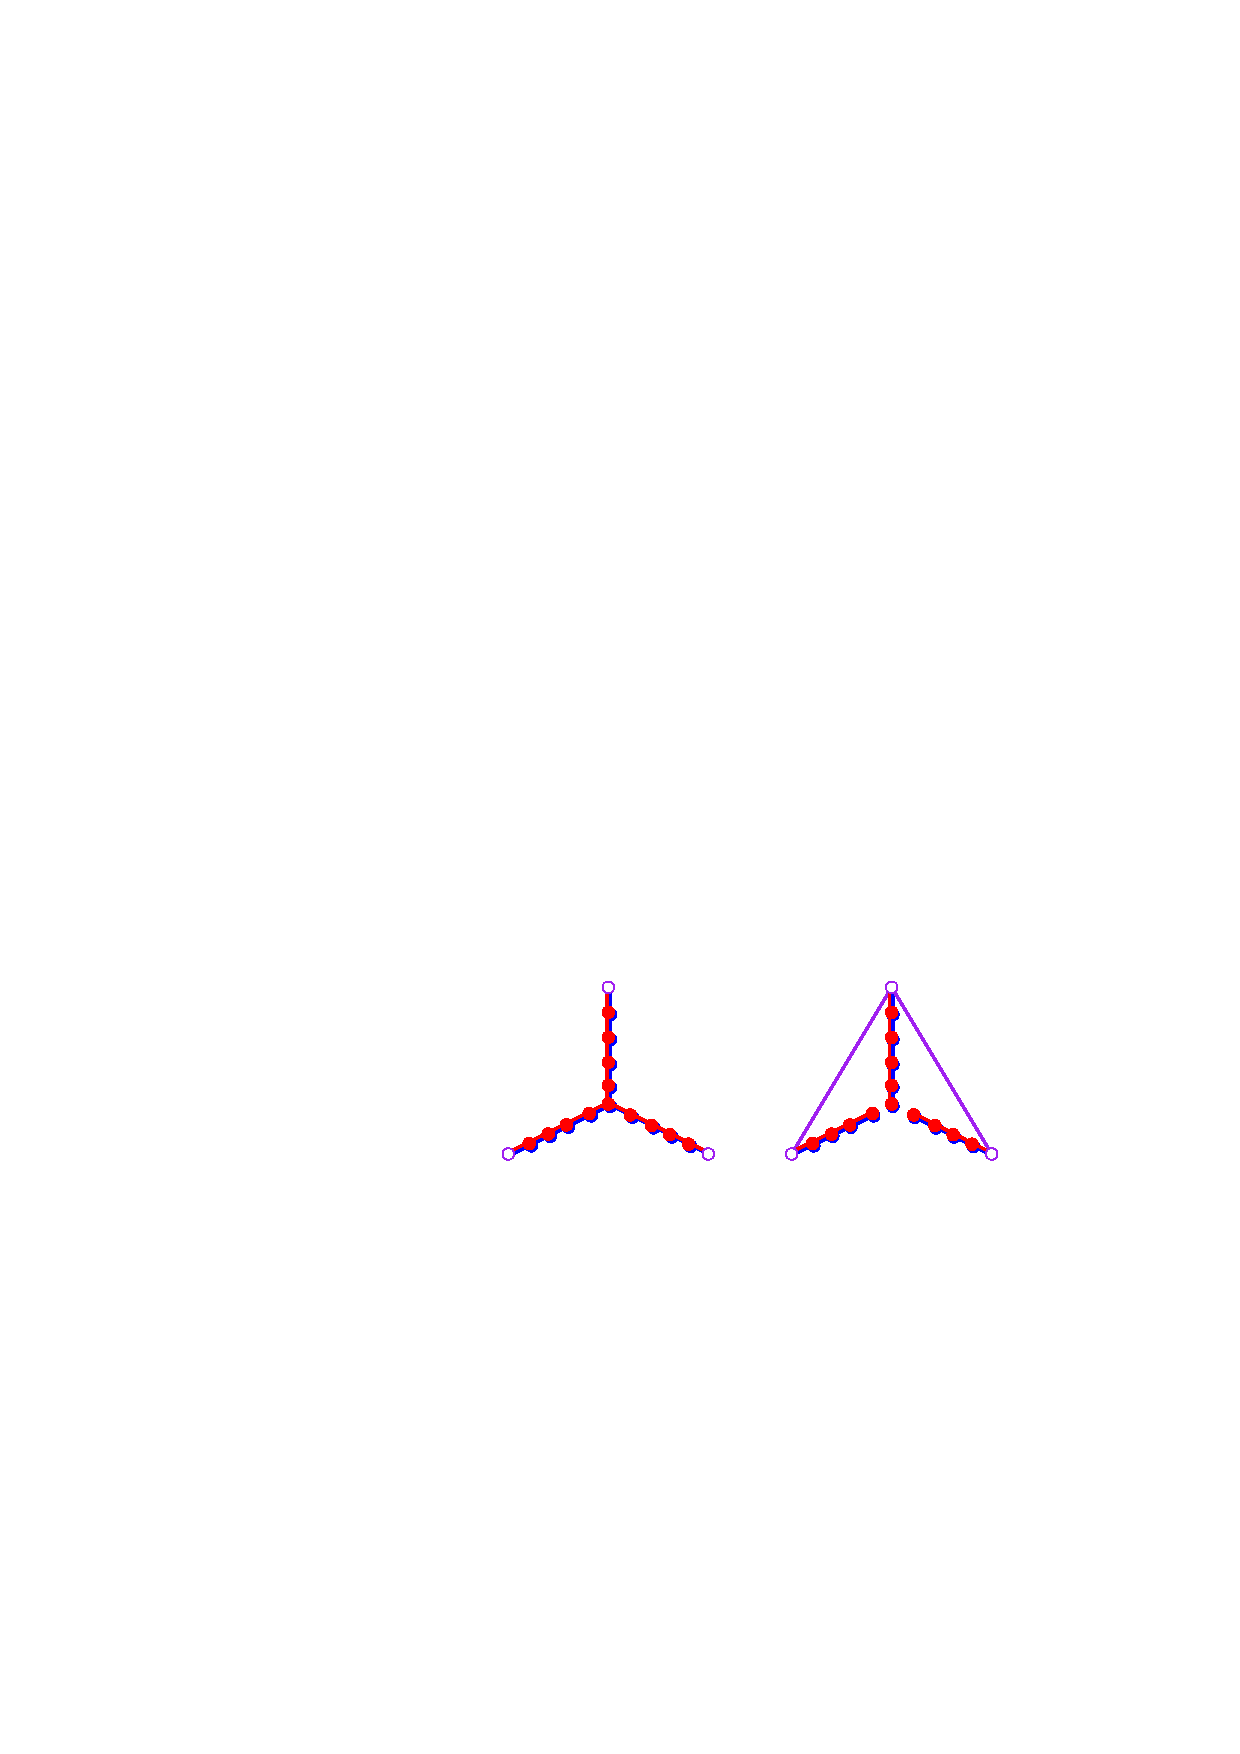
\includegraphics[width = 0.5\textwidth]{GD13_299-310_example.pdf}
    \caption{Taken from \cite{hurtado2016coloredspanninggraphsset}.}
    \label{fig:ambiguous}
\end{figure}
\paragraph{Clustering Vertices by Area}
Largely copied from the old graph harvester, this filter first clusters vertices by the size of the area they take up, then splits each cluster into two groups: the accepted group, and the group up for further examination.
If a cluster contains too few elements, or if its mean area is larger than the average over the remaining clusters, it would be sent to further examination, while other clusters would be accepted.
A cluster up for further examination then needs to ensure that it does not contain any center point from the set of already accepted vertices.
This check largely ensures that if there is one object for the outline and one for the interior of a vertex, just one, usually the interior due to its smaller area, is chosen.
However, the parameter of a minimum cluster size interestingly enough turned out to be a hugely influential parameter:
While I eventually got it down to a value of $3$, pushing it down further comes at a huge cost of detection rate, likely due to less actual vertices being accepted without any further examination.
This creates the opportunity for huge objects to get accepted as a vertex, if they are examined before any of the actual vertices that it overlaps.
That way, the huge vertex would remain accepted, and later merge with all actual vertices into one big vertex, swallowing parts of the actual graph drawing.
While I believe that there could be better ways to balance an initial selection of vertices, this one proved good enough, so that I found it hard to manually find an instance where this approach causes problems.


\paragraph{Height-to-Width Ratio}
Another filter that seemed promising at first was that of a filter based on the height to width ratio of a vertex.
I eventually optimized the parameter so that any vertex that has less than 75\% of its width in height, or of its height in width, would be rejected.
While this initially gave a small boost in recall, recent tests have shown no difference.
A further optimization could be to only use the filter, if some vertices still remain after, but in its current form, the impact of the filter seems to be weak.

\paragraph{Size of Vertex Compared to Total Size of Figure}
While simply filtering vertices if their area is too large relative to that of the figure seems like a good idea, in practice other filters already seem to do this job.
As a result, no difference in recall could be observed when changing the threshold for this variable within reasonable bounds. 
For example, filtering any vertex that takes up 20\% or more of the total area, compared to already filtering it if it takes up 5\% of the total area, does not change recall at all, and setting the threshold too low naturally hurts recall, rather than helping it.
However, one interesting observation is that contrary to intuition, the total number of detected graphs is higher with a stricter threshold: having detected a total of 611 graphs with a threshold of 5\% as opposed to just 578 graphs detected with 20\%.
This could indicate that there are some niche instances the old pipeline could not properly detect, that do rely on this filter, which motivated me to keep the threshold relatively low at 5\%.
%Probably has to do with the large vertices being merged with smaller ones, thus the total number of vertices goes down, below the threshold of 5


\paragraph{Brightness}
Filtering objects, not just vertices, by brightness could be a powerful tool to get rid of many objects that make an instance difficult to detect, such as grids and background colors.
For instance, \cref{fig:grey_background} shows a graph drawing with a light gray grid laying beneath.
Creating a brightness scale from 0 (black) to 1 (white) and completely throwing away any object over a certain threshold can make many instances easier.
For example, a threshold of $0.87$ would cause the aforementioned graph to lose its underlying grid.
However, overall $0.87$ seems like it is already too strict, as many instances such as the one shown in~\cref{fig:grey_vertex} break at this point as well.
In total, a threshold of $1$ compared to one of $0.87$ detects 222 as opposed to just 215 graphs from the data set, which unfortunately indicates that, while there is a trade-off of sacrificing some graphs to be able to detect others, it is generally not worth taking currently since it means losing graphs in total.
\begin{figure}
    \centering
    \begin{subfigure}{0.49 \textwidth}
        \centering
        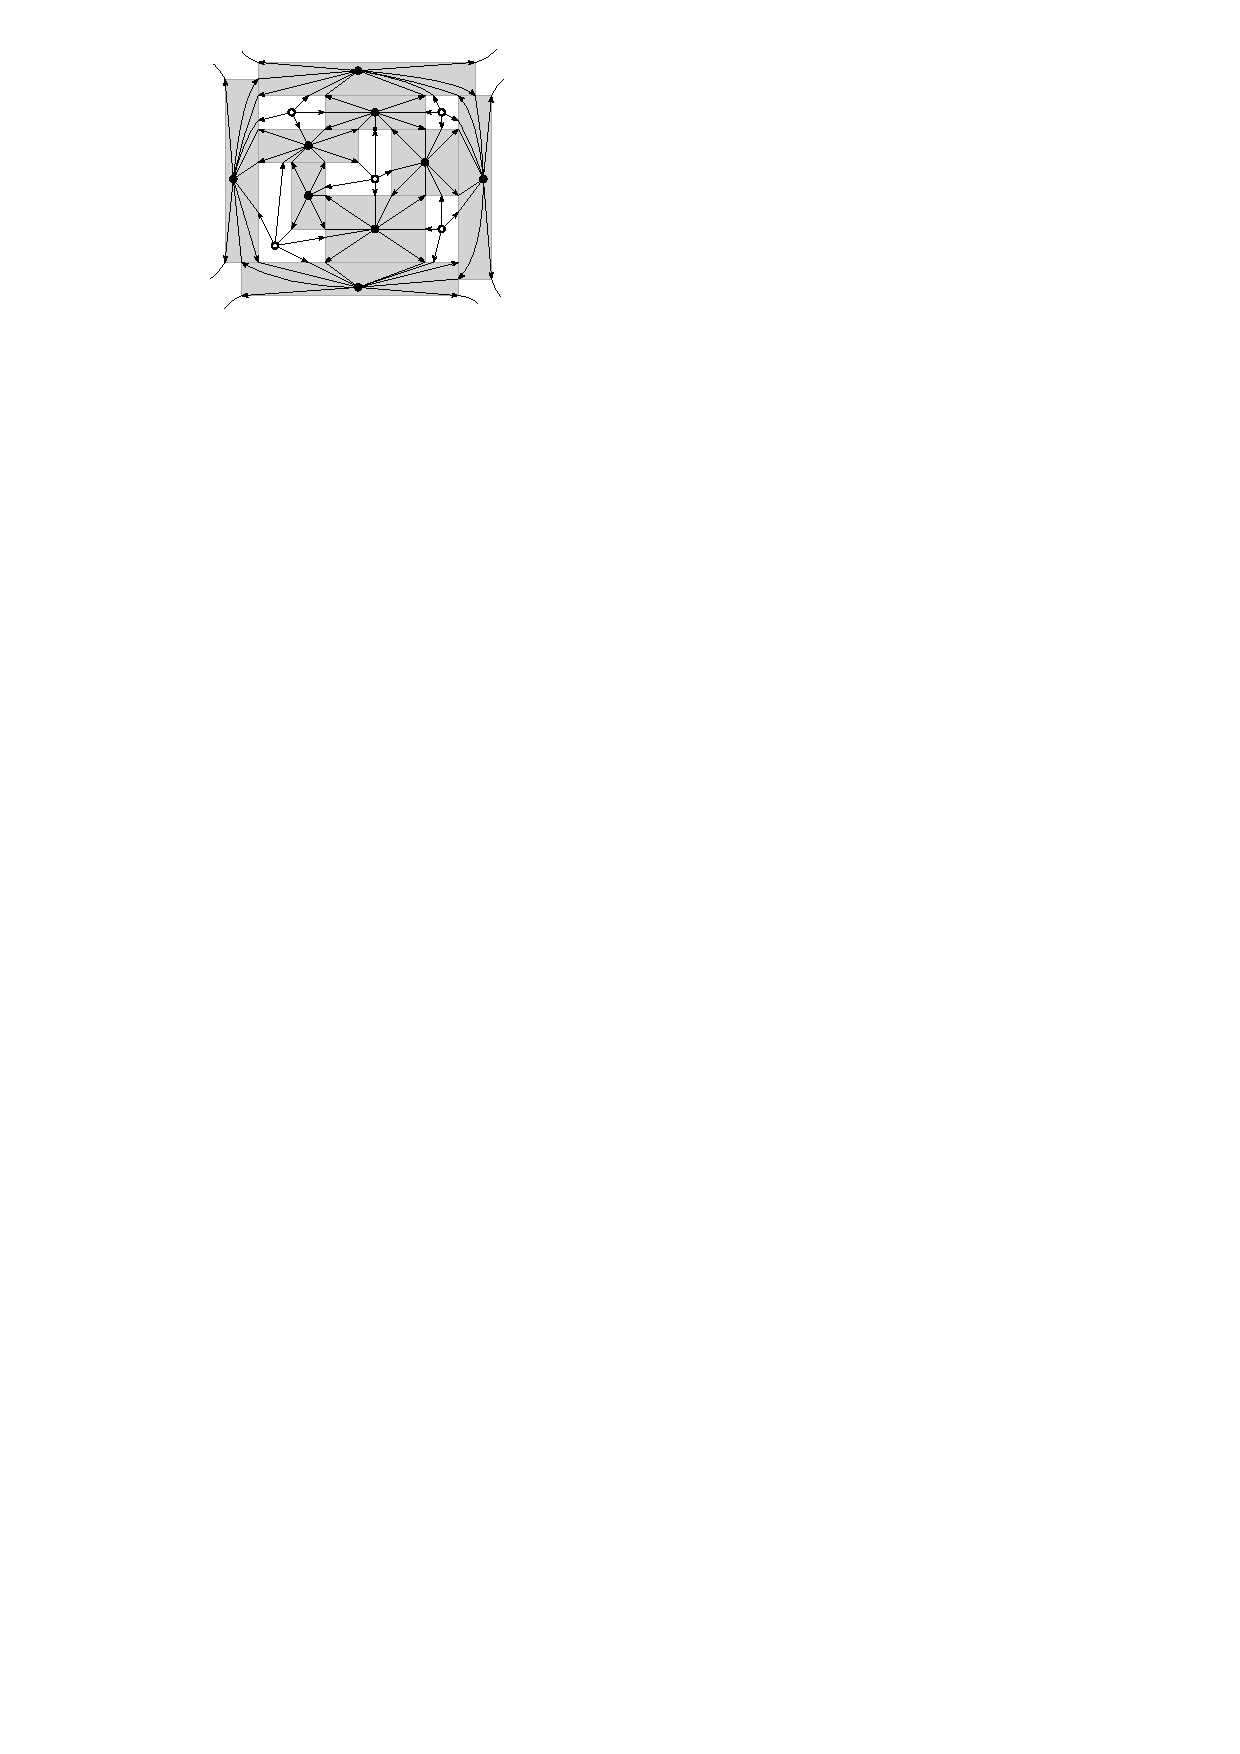
\includegraphics{GD15_243-256_example.pdf}
        \caption{Taken from \cite{klawitter2015combinatorialpropertiestrianglefreerectangle}.}
        \label{fig:grey_background}
    \end{subfigure}
    \begin{subfigure}{0.49 \textwidth}
        \centering
        
\includegraphics[page = 2]{GD20_56-70_example.pdf}
        \caption{Taken from \cite{bhore2020parameterizedalgorithmsqueuelayouts}.}
        \label{fig:grey_vertex}
    \end{subfigure}
    \caption{Two example graph drawings illustrating the dilemma of choosing a brightness threshold.}
\end{figure}

\paragraph{Arrows}
While the old implementation with its strict definition of a vertex had no problem with arrow heads, my new implementation does suffer from detecting any arrow head as a vertex, leading to many falsely detected instances.
To fix that, I implemented a simple arrow head detection, that would reject any object as vertex candidate, if it contains a sharp angle, namely 45° or less.
As a small optimization, the system actually does not compute the internal angles, but instead the cosines, where a cosine of $0.70710678118$ or larger corresponds to such an angle.


In order to compute the internal angles of an object, I simply do pairwise comparisons between any two strokes that meet in a common point.
With the first iteration of this algorithm simply walking along the outline of an object to find these pairs, I quickly encountered a bug that caused many arrow heads to not be detected.
The fix lied in the interesting observation, that some objects are actually drawn in a way where they close the loop through walking along the perimeter, and then close the loop again by connecting the first and last endpoint of the object's path.
Since those are already identical, this resulted in many arrow heads having one line segment of length $0$, so that if two adjacent line segments form a tight angle, that pair would never be checked because along its perimeter, a line segment of lenght $0$ lies between the two segments.


By fixing that bug, arrow head detection allowed correct detection of twelve additional instances, so that instead of $210$ graphs, $222$ could be found.

\subsubsection{Implied Vertices}
A large difference to the old pipeline is an attempt to detect implied vertices. 
To do that, I simply check for an instance if there are any vertex candidates left after initial filtering.
If not, the system will look for any point where three or more meet in an endpoint, and create a vertex incident to these edges at that position.
Eventually I tried creating implied vertices at a point even if just two edges meet there, but this caused hundreds of false positives due to any drawn object with at least six segments, such as letters, suddenly turning up as a detected graph, which led me to revert this decision.
However, none of the graphs with implied vertices are represented in the benchmark due to the old implementation not having this feature.
Determining the actual impact of the feature on the detection rate thus necessitates further manual evaluation.


\subsubsection{Graph Detection}\label{sec:graph}
With the set of vertices being determined, the next step is checking which edges are incident to that vertex.
Although most vertices lie on an endpoint of an edge segment, there are many instances where vertices lie between two endpoints, which led me to the following algorithm:


First, divide the segment into many sample points (my results come from using 30 points), with the first and last being the two endpoints and the others being equally spaced along the segment.
Secondly, check for each vertex if any sample points lie within its bounding box, scaled by some lenience factor (best results with $1.07$).
The concrete implementation of the range query is through RBush\footnote{https://github.com/mourner/rbush}.
The result is an incidence list of edge segments for every vertex that will afterwards be used to split every segment so that no segment has a vertex lying between its two endpoints, and every edge segment knows if it is incident to a vertex at each of its endpoints.
With an edge being a path from one vertex to another, there may be instances where multiple vertices are incident to a single endpoint.
In such a case, I take the vertex minimizing the distance to the endpoint, which is a solution that seemingly has not caused any problems.


After that, I use KDBush\footnote{https://github.com/mourner/kdbush} to find all orphaned edge endpoints incident to another orphaned edge endpoint, i.e.~a pair of incident endpoints that are both not incident to any vertex.
Note that while the previous model only links edge segments if they do not form a tight angle (60° or less), I have not implemented this check.
While the search radius has caused some troubles, the best results could be achieved with the search radius being either the stroke width, or 0.25px, depending on which is larger, with very short segments not getting the guarantee of at least 0.25px.
This solution seems able to handle two specific edge cases that were particularly prevalent:
One occurs in instances where two strokes form one edge, yet they don't exactly meet in a given point, i.e.~there is an offset between two consecutive edge segments (see~\cref{fig:too_narrow}).
The other occurs whenever two separate edges come very close to each other at a given endpoint, which might cause the wrong edge segments to be linked to each other (see~\cref{fig:too_wide}). 
\begin{figure}
    \centering
    \begin{subfigure}{0.49\textwidth}
        \centering
        
\includegraphics{search_radius_too_narrow.pdf}
        \caption{The two orange segments should be linked, yet a search radius that is too small will not connect the two segments into one edge.}
        \label{fig:too_narrow}
    \end{subfigure}
        \begin{subfigure}{0.49\textwidth}
        \centering
        
\includegraphics{search_radius_too_wide.pdf}
        \caption{The purple segments should be linked, yet a too large search radius might cause one of them to connect to the orange clutter instead.}
        \label{fig:too_wide}
    \end{subfigure}
    \caption{Two examples that highlight why choosing a search radius can be tricky.}
\end{figure}


This allows chaining different segments together into one large edge, which is important for many instances: 
in an earlier version where this was not possible, only 22 out of the 248 `A' graded graphs could be matched.
After implementing the chaining of edge segments, the recall jumped up by a relative 36\%, up to a total of 30 matched instances.



Lastly, remaining half orphans are rescued by linearly extending them into the direction they point at. 
For Bézier curves, the extension goes into the direction obtained by shooting from the last control point towards the orphaned endpoint. 
Since this implementation also caused many false positives, I had to carefully limit the extension, up to a maximum of 30 pixels, or seventeen percent of the edge segment's length.
During tuning of these parameters, it turned out that the relative extension threshold is much more limiting than the absolute one: 
Although there were two instances that could only be detected with at least three pixels of absolute extension, and one that needed nine pixels, any increase beyond that neither positively nor negatively influenced the detection rate.


The resulting incidence list can then be turned into a graph using depth-first-search, just like the old graph harvester did.

\section{Limitations and Possible Solutions}
\paragraph{Arrow Head Detection}\label{sec:arrows}
The system currently relies on reusing arrow heads as edge segments.
This causes many perfectly fine edges to attach the arrow's stroke segments to its end, rather than the vertex it is incident to.
While that does not cause any problems in itself, it causes the last segment of the edge to be very short.
That way during the edge extension process for half-orphans, the relative edge extension threshold causes many segments to be extended much less than they could be.
Thus getting rid of arrows being used as edge segments could be the key to detecting more graphs accurately.

However, in order to enable that, it would be interesting to analyze cases where an arrow is actually important for edge detection.
Possible indicators could be size of the arrow, and number of vertices it is incident to. 
For example, if the arrow consists of three line segments, there could be three vertices the arrow is incident to. 
If there are more or less vertices in its vicinity, the arrow might be safe to discard as an edge.

\paragraph{Large Vertices}\label{sec:large}
The implementation often bloats vertices up to be much larger than they appear to be in the original drawing, causing problems by finding additional incident edges and falsely merging two bloated vertices into one.
It remains to be seen if this is due to a bug, or some other phenomenon that can be counteracted.
A plausible explanation could be, that some papers might draw their vertices with a blown up interior that they then clip to the outline of the vertice.
Since clipping paths are not considered, that blown up interior stays as large, and might be able to sneak through the filters designed to catch large vertices.
%%%%%%%%%%%%%%%%%%%%%%%%%%%%%%%%%%%%%%%%%%%%%%%%%%%%%%%%%%%%%%%%%%%%%%%%%%%%%%%%
\clearpage
\bibliographystyle{mybabalpha-fl}
\bibliography{mybib}


\end{document}
